\documentclass{article}
\usepackage[utf8]{inputenc}
\usepackage[ngerman]{babel}
\usepackage{graphicx}

\title{Computergrafik Projekt}
\author{Projektgruppe "Zahnradapparatus" }
\date{Juni 2019}

\begin{document}

\begin{titlepage}
\maketitle
\end{titlepage}

\tableofcontents

\newpage

\section{Projektidee festlegen}
Nach Sichtung des bereits behandelten Vorlesungsmaterials hat sich die Gruppe dazu entschlossen, für das Projekte eine kleine Menge an selbsterstellten Zahnrädern für das Projekt zu entwerfen. 
Es war geplant, dass diese Zahnräder gemäß den bereits bearbeiteten Übungen an unterschiedlichen Koordinaten im Raum platziert werden und sich dort, ineinandergreifend, bewegen. 

Geplant ist die Umsetzung von zwischen 3 und 5 Zahnräder mit verschiedenen Größen und farblichen, sowie texturellen Differenzen, die durch Keyboardeingaben gesteuert werden können. 

Es sollen dabei alle in der Vorlesung angesprochenen Themenbereiche Anwendung finden. 
Der Einfachheit halber sollten diese einzelnen Teilaspekte in der Reihenfolge eingebaut werden, wie sie auch gemäß der Veranstaltung vorgestellt werden. 



\subsection{Konkretisieren der Projektidee}
Nach Bekanntgabe der genaueren Anforderungen an das zu erstellende Projekt wurde ein erstes Teammeeting angesetzt, um zu besprechen, wie deren Realisierung konkret aussehen könnte. 
Gemeinsam hat sich die vierköpfige Gruppe nach einiger Diskussion auf eine Idee geeinigt, die sowohl alle Anforderungen an das Projekt erfüllt, als auch im Rahmen der Fähigkeiten und Kenntnisse der einzelnen Gruppenmitglieder im angegebenen Zeitrahmen umsetzbar erscheint. 

Es wurde sich darauf geeinigt, dass zuerst gemeinsam ein Prototyp eines selbst modellierten Zahnrads gebaut werden sollte. 
Die Wahl auf das Zahnrad fiel aufgrund von unterschiedlichen Überlegungen:

\begin{itemize}
    \item Das Zahnrad selbst erscheint in seiner geometrischen Modellierung einmalig aufwendig, jedoch in seiner Schwierigkeit dem Projektumfang angemessen. 
    \item Die Zahnräder können ineinander verbaut werden, sodass ein "Kurbeln" an einem Zahnrad den gesamten Apparatus in Bewegung setzt. *
    \item Man kann den einzelnen Zahnrädern unterschiedliche Größen geben, sodass unterschiedliche Skalierungsmatritzen auf das originale Objekt angewendet werden. *
    \item Man kann den einzelnen Zahnrädern unterschiedliche Texturen / Farben / Lichtrefkletionsmodelle geben und so visuell ansprechende Effekte erzielen. 
    \item Man kann die einzelnen Zahnräder an unterschiedlichen Raumkoordinaten positionieren, sodass unterschiedliche Transformationen am originalen Objekt vorgenommen werden. 
\end{itemize}

Bedingt durch die Möglichkeit,den Apparatus durch Drehung der Zahnräder in Bewegung zu setzen, würde das Projekt dementsprechend auch eine dynamisch-animierte Komponente enthalten, die sich die Gruppenmitgleider ausdrücklich gewünscht hatten. 

Weiterhin bot die Idee des Zahnradapparatus' die Möglichkeiten, diesen durch eine dynamische (keyboard-gesteuerte) Implementierung zu \enquote{umschreiten}, um den Apparat von unterschiedlichen Seiten zu betrachten. 

Nachdem sich alle Gruppenmitglieder mit dem Vorschlag des Zahnradapparatus' einverstanden erklärt hatten, erfolgte die Vorstellung der Idee vor dem Dozenten, der mit dem Umfang und den Implementierungen des Projektes einverstanden war. 



\paragraph{*Anmerkungen}
Die vordergründigen Überlegungen zu den einzelnen Gründen für die Implementierung eines Zahnradaparatus haben sich im Laufe der Vorlesung als missverständlich erwiesen. 

So ist es nicht ohne weiteres möglich, dass ein "Kurbeln" an einem Objekt ein anderes Objekt in Bewegung versetzt. 
Eine Implementierung dieser Funktion hätte vorgenommen werden können, war jedoch im gegebenen Zeitrahmen und Umfang des Projekts mit dem bisherigen Kenntnisstand der Gruppe nicht möglich. 
Retrospektiv könnte dies heute, würde noch einmal ein neues Projekt aufgesetzt werden, umgesetzt werden. 

Parallel ist es nicht möglich, den Zahnrädern ohne weiteres unterschiedliche Größen zu geben, bzw. dasselbe Objekt durch Skalierung zu einem größeren / kleineren Zahnrad zu machen. 
Hintergrund ist hier (logischerweise), dass sich bei einer Größenänderung von einem Zahnrad zwar die Größe (Durchmesser bzw. Radius) des Rades ändert, jedoch die Größe der einzelnen Zähne gleich bleiben muss, damit diese lückenlos ineinander greifen können. 

Dies bedeutet somit, dass für ein kleineres Zahnrad ein neues Modell erstellt werden muss, dass nicht nur einen kleineren Radius besitzt, sondern auch weniger Zähne gleicher Größe auf dem Modell unterbringt ( s. \ref{fig:littleGear}). 

\begin{figure}
\centering

\includegraphics[scale=1.7]{Little_Gear}
\caption{Zahnrad bei Verkleinerung des Radradius}
\label{fig:littleGear}
\end{figure}



\section{Arbeitsumgebung einrichten}



\subsection{Git}
Um die Zusammenarbeit aller Gruppenmitglieder angemessen koordinieren zu können, sowie um praktische Erfahrungen mit einem Version-Controll-System zu sammeln, entschloss sich die Gruppe, Git zu benutzen. 

Nachdem ein gemeinsames Repository aufgesetzt und allen Mitgliedern Zugriff darauf gewährt wurde, war jedes Gruppenmitglied nun unabhängig voneinander in der Lage, den aktuellen Code von Github herunterzuladen, bzw. eigene Änderungen am Projekt in das Repository zu pushen, um sie für alle verfügbar zu machen. 

Die Arbeit mit Git (über den Dienst Gitkraken) erwies sich im Verlaufe des Projektes generell als sehr lehrreich. 
Die Einarbeitung in die Funktionsweise von Git stellte allerdings, insbesondere am Anfang, einige Schwierigkeiten dar. 

Allgemein kann jedoch generell geschlossen werden, dass, je mehr Kenntnisse die Gruppe im Umgang mit Git sammeln konnte, desto stärker dessen Vorteile in den Vordergrund traten.  

Generell überwogen für alle Beteiligten die Vorteile einer sinnvollen Möglichkeit zur Versionskontrolle über die anfänglichen Schwierigkeiten bei der Einarbeitung in die Thematik.


\subsection{Eclipse}
Weiterführend musste auf allen Rechnern der Gruppenteilnehmer Eclipse, bzw. die korrekte Version von Eclipse installiert werden, sowie der Szenegraph aus den Veranstaltungsübungen kompiliert und zum Laufen gebracht werden. \label{EclipseProbleme}

Dies war am Anfang mit einigen Schwierigkeiten verbunden. 
Die Schwierigkeiten entstanden teilweise aus den unterschiedlichen Hardwarevoraussetzungen der einzelnen Rechner - \textit{zwei Gruppenmitglieder haben sich im Verlaufe des Projekts einen neuen Laptop angeschafft, da die Kompilierung und Ausführung der Projekte teilweise wahrscheinlich hardwarebedingt nicht unterstützt werden konnte} - teilweise bedingt durch Softwaredifferenzen (Linux vs. Windows, bzw. den Einstellungen von Eclipse allgemein) und teilweise aufgrund einer schmalen Dokumentation der verwendeten Ressourcen. 



\section{Erstes Zahnradmodell erstellen}
Für eine erste Implementierung der Idee in Form eines Minimal-Viable-Products (kurz: MVP) wurde gemeinschaftlich ein Zahnradmodell erstellt. 

Die nötigen Vertices und Faces wurden dabei, in Ermangelung von Kenntnissen im Bereich Blender, noch von Hand berechnet und hart im Code eingeschrieben. 

\begin{figure}
\centering
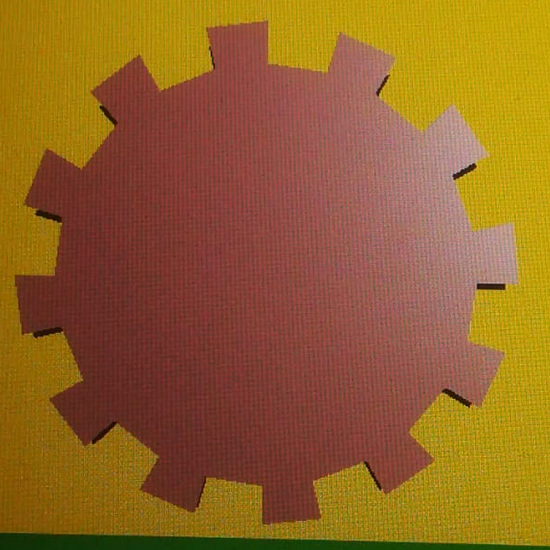
\includegraphics[scale=1.0]{Gear.png}
\caption{Einfaches, selbst erstelltes Zahnrad}
\label{fig:gear}
\end{figure}

\subsection{Blender}
Es sei an dieser Stelle angemerkt, dass es sich für künftige Veranstaltungen anbieten würde, die Ausführungen zu Blender und .Obj-Dateien inhaltlich vorzuziehen. 

Die Erstellung des Zahnradmodells hat einen enormen Zeitaufwand für alle Gruppenmitglieder bedeutet - neben den eigentlichen Berechnungen und dem aufwändigen händischen Einpflegen der einzelnen Koordinaten in den Source-Code, waren zudem bis zur Verwendung von .Obj-Dateien immer wieder unerklärliche Bugs im Modell zu finden, die sich auf die Darstellung, Beleuchtung und Animation bezogen haben. 

Dies war auch der Grund dafür, dass letztendlich (nach Behandlung der Inhalte in der Veranstaltung) der Umschwung vom eigenen Modell hin zu Blender-generierten .Obj-Dateien stattgefunden hat. 
Parallel schlug es allerdings auf die grundlegende Motivation der Gruppe, dass der Teil der Gruppenarbeit, der als am Zeitaufwändigsten empfunden wurde, sich im weiteren Verlaufe der Veranstaltung als vollständig überflüssig erwies. 
\newpage

\begin{figure}[h!]
\centering
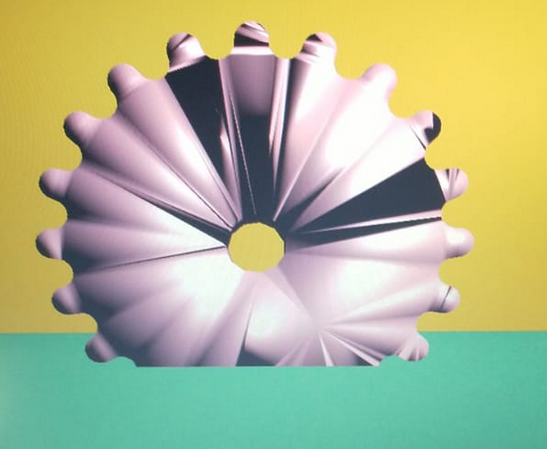
\includegraphics[scale=1.0]{Buggy_Gear1.png}
\caption{Probleme im eigenen Zahnradmodell}
\label{fig:bugGear1}
\end{figure}

\begin{figure}[h!]
\centering
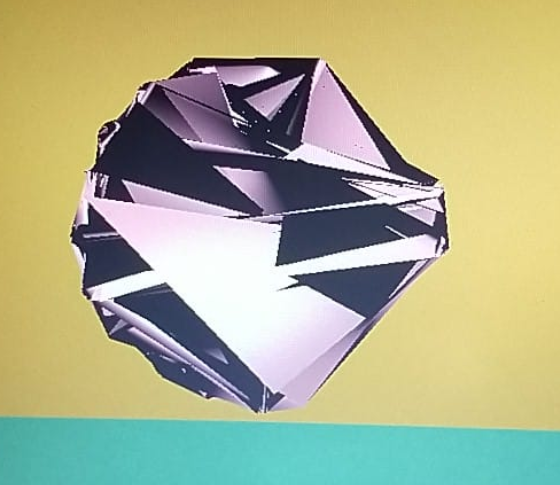
\includegraphics[scale=1.0]{Buggy_Gear2.png}
\caption{Noch mehr Probleme im eigenen Zahnradmodell}
\label{fig:bugGear2}
\end{figure}

\subsection{Erste Probleme}
Parallel sah sich die Gruppe mit der ersten Herausforderung in diesem Projekt konfrontiert: 
Die Arbeitsumgebung aus den Übungen auf den einzelnen Privatrechnern der Mitglieder zu konfigurieren, sodass das Basisprojekt kompiliert und gestartet werden konnte. 
Obwohl dies eigentlich eine grundsätzliche Voraussetzung für die Weiterarbeit am Projekt ist, wurde insgesamt ein unverhältnismäßig großer Zeitaufwand für das Aufsetzen der Entwicklungsumgebung verbraucht (Näheres hierzu im vorigen Unterkapitel \enquote{Eclipse} \ref{EclipseProbleme}). 



\section{Raum + Interaktion}
Sobald die Entwicklungsumgebung auf allen Teilnehmerrechnern einsatzbereit war und parallel das erste Modell eines Zahnrads erstellt und in Github gepusht wurde, konnten die restlichen Teilnehmer damit beginnen, den aktuellen Stand zu pullen, um selbst weitere Modifikationen vorzunehmen. 

Um eine schnellere Bewältigung der noch ausstehenden Arbeitspakete zu ermöglichen, wurde aus diesem Grund eine Aufteilung der anstehenden Arbeitspakete beschlossen. 
Ein Arbeitspaket war die Erstellung des Raumes selbst. 
Ein weiteres Arbeitspaket war der Einbau des Zahnrads in den Raum. 

Final sollte ein erstes Interagieren mit den implementierten Objekten ermöglicht werden, sodass tastaturielle Kontrolle über das Objekt ausgeübt werden kann. 



\subsection{Raum erstellen}
Gemäß den Materialien, die durch die Übungen parallel zur Veranstaltung bereit gestellt wurden, konnte aus diesen das ursprüngliche Erstellen eines Raums abgeleitet werden. 

Sobald die Übungsaufgaben erfolgreich bearbeitet und dadurch das allgemeine Vorgehen hinreichend logisch verstanden worden war, konnte eine 1:1 Umsetzung der erlernten Inhalte auf das Projekt abgebildet werden. 



\subsection{Zahnrad in Raum einfügen}
Nachdem der grundlegende Raum vorhanden war, in dem sich das Projekt abspielen sollte, konnte damit begonnen werden, das Zahnradmodell in diesen einzufügen. 
In erster Instanz wurde dabei der Mittelpunkt des Raumes als Nullpunkt der Raumkoordinaten definiert. 

Sodann war es möglich, nicht nur das Zahnradmodell ebenfalls im Mittelpunkt des Raumes darzustellen, sondern dieses über Translation und Rotation beispielsweise auch an eine der Raumwände \enquote{anzuhängen}. 

Zu diesem Zeitpunkt offenbarten sich auch die ersten Probleme mit dem selbsterstellten Zahnradmodell. 
Bei der Anbringung an die Raumwand kam es zu Fehlern in der Oberflächendarstellung, sowie beim ersten Versuch einer drehenden Animation zu Problemen beim Rendering des Animationsablaufs. 
Da die Lösung über den Einsatz von Blender noch nicht in Aussicht stand, wurde hierf+r ein weiterer großer Anteil der Projektzeit in das Korrigieren dieses Fehlverhaltens, sogar in das Erstelen eines gänzlich neuen Modells, verwendet. 



\subsection{Kamerasteuerung}
Da die Kamerasteuerung im vorgegebenen Arbeitspaket als "nicht intuitiv" empfunden wurde, beschloss die Gruppe, diese generell umzukehren. 

Durch eine Invertierung der Kamerasteuerung konnte erreicht werden, dass sich die Steuerung der Kamera für den User \textit{natürlicher} anfühlte, sodass direkter mit dem Projekt interagiert werden konnte und keine Zeit für ein Einfinden in die Steuerung des kompilierten Programms verwendet werden musste. 


\subsection{Fertigstellung der Arbeitspakete}
Sobald die Arbeitspakete "Raumerstellung", "Zahnradeinbindung" und "Kamerasteuerung" grundlegend implementiert waren, konnten neue Arbeitspakete erstellt werden. 
Um die gewonnenen Kenntnisse aus den Arbeitspaketen zu teilen, wurden die Ergebnisse und Vorgehensweisen der Gruppenmitglieder untereinander vorgestellt. 
So hatte jedes Mitglied, auch wenn eine Arbeitsteilung stattgefunden hatte, in etwa denselben Wissenstand über die Vorgänge im Projekt. 

Nachdem die grundlegenden Probleme in der Darstellung des Zahnradmodells zwischenzeitlich beseitigt worden waren, konnte ein weiterer Arbeitsschritt implementiert werden: 
das Einfügen eines zweiten Zahnrads, dass neben dem bestehenden Zahnrad platziert wurde. 
Die Umkehrung der Drehrichtung und eine bei beiden Modellen gleiche Drehgeschwindigkeit sorgte folgend dafür, dass die Zähne der einzelnen Zahnräder fließend ineinander griffen. 

Der erste Prototyp des Zahnradapparatus' präsentierte sich beeindruckend, trotz weiterhin bestehender, jedoch marginaler Darstellungsfehler. 





\section{Licht, Raum + Bewegung}



\subsection{Beleuchtung}
Da die Steuerung der Kamera aus den bereitgestellten Arbeitsmaterialien sich immernoch  etwas kontraintuitiv gestaltete, wurde auch hieran weitergearbeitet. 
Die Pfeiltasten nach vorne, hinten, links und rechts sorgten somit nun für eine Bewegung in die entsprechende Richtung, "q" und "e" ermöglichten ein Drehen der Kamera um sich selbst. 

Für die Arbeit an den Zahnradmodellen, die noch einige Schönheitsfehler enthielten, wurde mit den Tasten "x" und "v" die Möglichkeit geschaffen, links-/rechtsdrehend um ein Objekt zu "fahren", sodass die Beleuchtung stationär an Ort und Stelle stehen bleibt und sich nur die Kamera um das Objekt bewegt. 

\paragraph{Anm.d.A.: 
Die hier gemachten Angaben beziehen sich noch auf einen Zwischenstand im Entwicklungsstadium des Projekts. 
Die final implementierten Steuerungstasten finden sich in der dem Projekt beiliegenden Readme-Datei. 
}



\subsection{Zahnradmodell aus Blender}
Da nach wie vor und trotz hartnäckigen Lösungsversuchen immernoch Darstellungs-, Textur- und Animationsprobleme bei der Verwendung des eigenen Zahnradmodells bestanden, arbeitete sich ein Gruppenmitglied kurzerhand in die grundlegendsten Befehle und Funktionsweisen der Grafiksoftware \enquote{Blender} ein. 
Nach dem Erlernen der grundlegendsten Funktionen war es dem Gruppenmitglied daraufhin möglich, in Blender ein neues Zahnradmodell zu erstellen. 

Dieses präsentierte sich nicht nur in seinem Detailreichtum beeindruckend, sondern löste über die Export-Funktion als .Obj-Datei auch die Probleme, die bislang am selbsterstellten Modell bestanden haben. 

Um die exportierte Datei folgend noch vom Projekt lesbar zu machen, bzw. generell eine Möglichkeit zu schaffen, diese in das Projekt zu laden, wurde ein .Obj-Reader implementiert. 

Nach einige wenigen gescheiterten Experimenten am Source-Code gelang es schließlich, in einem wesentlich kleineren Zeitrahmen, als die Erstellung des erstes Zahnradmodells gekostet hatte, ein hochwertiges Zahnradmodell in Form von einer detailreichen Uhr nicht nur zu erstellen, sondern auch noch in das bestehende Programm einzupflegen. 

%\newpage

\begin{figure}[h!]
\centering
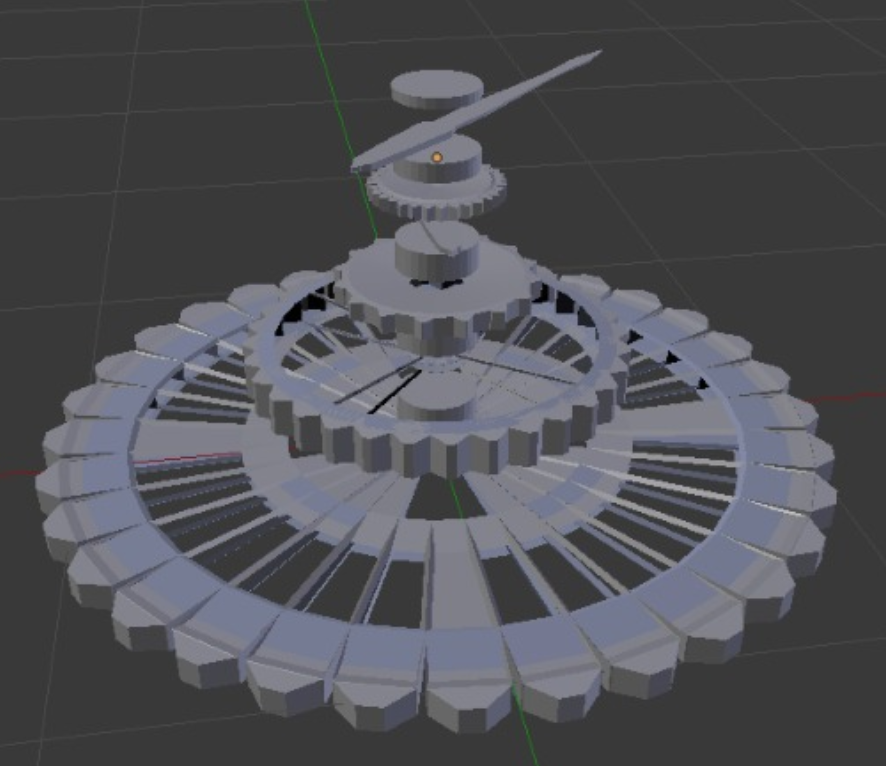
\includegraphics[scale=0.7]{Final_Clock_Blender.png}
\caption{Zahnradmodell nach der Nutzung von Blender}
\label{fig:clock_blender}
\end{figure}

Das fertige Ergebnis, eingespeist in das bisherige Projekt und veredelt durch eine gold- und messingfarbene, metallerne Oberfläche, übertraf alle bisherigen Erwartungen in seiner Schönheit und Eleganz. 

\begin{figure}[h!]
\centering
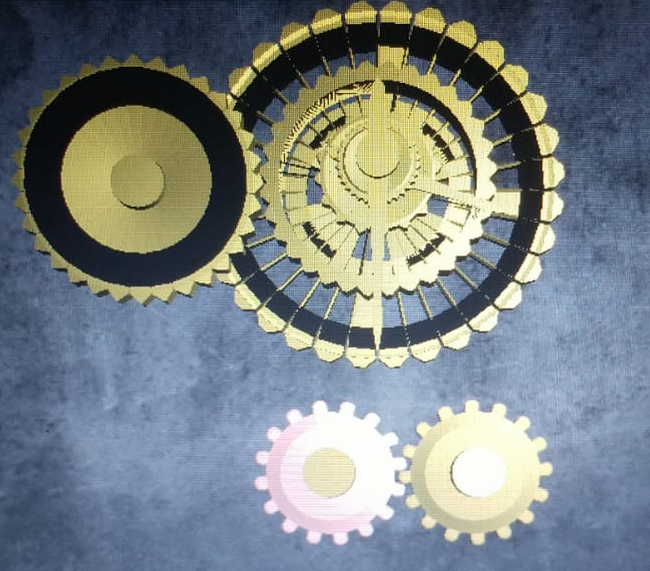
\includegraphics[scale=0.8]{finalClock.png}
\caption{Blender-Uhr im Projekt}
\label{fig:finalClock}
\end{figure}

Parallel war während den Arbeiten an dem Modell und der Kamerasteuerung an der Implementierung einer Textur für das Objekt geforscht worden. 
Ein erster Anlauf war die Implementierung von einfachen 2D-Bild-Texturen auf die vorhandenen Raumwände, die durch ihre Natur relativ einfach mit einer Textur versehen werden konnte (im Gegensatz zu beispielsweise dem eigens-modellierten Zahnrad). 

Von der Implementierung einer Textur für das Zahnrad wurde aus zwei Gründen abgesehen: 

\begin{itemize}
    \item A) Die Erstellung einer entsprechenden Textur für eine so filligrane Form wie das Zahnradmodell wurde als zu aufwändig gemessen am Zeitrahmen des Projekts erwogen. 
    \item B) Die metallerne Oberfläche des Zahnrads wurde von sämtlichen Projektteilnehmern nicht nur als grundlegend sehr ästhetisch empfunden, sondern entspricht auch der Darstellung eines Zahnrads, wie sie in der Realität tatsächlich auftritt. 
\end{itemize}

Parallel wurde die Erstellung und der Einbau eines blendermodellierten, industriell-angehauchten Fenstergitters in Erwägung gezogen, dass als zweite Beleuchtungsquelle dienen könnte. 

In Kombination mit einer Zementtextur für die Wände würde das dem dargestellten Raum einen besonderen, industriellen Flair geben. 

Sodann konnten weitere Aufgabenpakete für das Erreichen des Projektziels abgeschätzt werden: 
Eines dieser Aufgabenpakete war die Erstellung zweier leuchtender Sphären, damit das Projekt zwei Lichtquellen  enthält. 
Die Entscheidung über das genaue Design dieser Sphären wurde bis nach der Fertigstellung des Aufgabenpakets aufgeschoben, damit ein möglichst großer kreativer Freiraum für die Gestaltung des Raums um den Zahnradapparatus garantiert werden konnte. 

Eine weitere Aufgabe war die Implementierung einer Taste, die die Drehung der Zahnräder ineinander starten oder beenden sollte. 
Dies würde nicht nur die Interaktion mit dem Projektmodell ermöglichen, sondern auch die gewünschte Animation der dargestellten Objekte vervollständigen. 

Weiterfolgend hat die Gruppe in Erwägung gezogen, eine Restriktion der Kamera zu implementieren, damit man nicht versehentlich über die Steuerung mit den Pfeiltasten aus dem Raum heraus navigieren könnte. 
Im Gespräch mit dem die Veranstaltung begleitenden Dozenten wurde jedoch beschlossen, dass es sich hierbei um keine grundlegende Anforderung handelt und die Implementierung voraussichtlich einige Komplexität mit sich bringen würde.

Da diese Erwägung somit nicht zum Bestehen des Projekts vorausgesetzt wurde,  wurde die Kamerarestriktion vorerst auf die "Wunschliste" gestellt: 
Eine Liste, mit Wünschen, Ideen und Anregungen der Gruppenteilnehmern, die "nice to have" wären, allerdings nicht im Rahmen des Projekts als zwangsläufig notwendig erachtet wurden. 
Eine Umsetzung dieser Liste sollte gegen Ende des Projekts evaluiert werden, falls die Abgabeziele vor Ende der Projektzeit erreicht würden und die Projektteilnehmer sich folglich freiwillig weiter mit der Materie beschäftigen wollten. 





\section{Mehr Licht, Tastendruck, Aufräumarbeiten}
Um final die Anforderungen an das Projekt zu erfüllen, waren noch zwei Aspekte der grundsätzlichen Aufgabenstellung offen. 
Es handelt sich dabei um 
\begin{itemize}
    \item die Verwendung einer zweiten Beleuchtungsquelle und
    \item die Interaktion mit einem Objekt. 
\end{itemize}

\subsection{Zweite Lichtquelle}
Im Verlauf des Projekts hat sich die Gruppe entschlossen, als zweite 
Lichtquelle kleine Lichtspots zu verwenden, die an den Raumwänden platziert werden sollen. 

Die im Vorfeld erwägten Sphären, bzw. der Einsatz eines Fenstergitters waren zwischenzeitlich wieder verworfen (Spähren), bzw. auf die \enquote{Wunschliste} (Fenstergitter) gestellt worden. 
Hintergrund dieser Entscheidungen waren Probleme beim generellen Verwenden einer zweiten Beleuchtungsquelle. 

Die Lösung dieser Problematik zeigte sich im weiteren Verlauf dadurch, dass die zweite Lichtquelle als Kindknoten der ersten Lichtquelle eingesetzt werden musste, und im Szenegraphen nicht beide auf einer Ebene stehen durften. 

Die Entscheidung zu den Lichtspots wurden nach einem Gespräch mit dem Dozenten gefällt, da dieser die Gruppe darauf aufmerksam machte, dass die dazu notwendigen Methoden bereits im zur Verfügung gestellten Szenegraphen implementiert waren. 



\subsection{Objektinteraktion}
Als Interaktion wurde nach Absprache mit dem Dozenten die Idee angenommen, die Drehungen des Zahnrads per Tastaturdruck zu stoppen, bzw. zu starten. 

Auf diese Weise sollte das gesamte Projekt zudem eine interaktive Komponente erhalten, die es einem Betrachter ermöglichen sollte, selbst auf das dargestellte Geschehen einzuwirken, anstatt dieses nur zu betrachten. 

Somit gestaltete sich diese Interaktion als weiteres Aufgabenpaket, dass es bis zur finalen Abgabe zu ermöglichen galt. 



\subsection{Restrukturierung des Szenegraphen}
Beim versuch, die letzten Arbeitspakete zu implementieren ist ein grundlegendes Hindernis immer deutlicher zu Tage getreten: 

Die Interaktion mit dem Objekt, die bislang immer wieder gescheitert ist, sowie die Implementierung der zweiten Lichtquelle erforderten eine Restrukturierung des bislang verwendeten Szenegraphen. 

Diese Erkenntnis schlug sich erneut massiv auf die Motivation der Gruppe nieder, da dies eine schwerwiegende Änderung in der bisherigen Funktionsweise des Projekts bedeutete. 

Gemeinsam, und unter erneutem großen zeitlichen Aufwand, gelang jedoch auch final die Überwindung dieses Hindernisses und die Freude war groß. 

Endlich war es möglich, sowohl die Interaktion per Tastendruck einzupflegen, als auch eine zweite Beleuchtungsquelle anzubringen. 

Die Interaktion von Wänden, Licht und Zahnrädern lief dabei endlich wie geschmiert. 
Anscheinend war ein großer Anteil der bisherigen Problematiken durch eine bizarre Strukturierung des Szenegraphen ausgelöst worden. 
Da dieser Knoten nun geplatzt war, schritt die Fertigstellung des Projektes mit großen Schritten voran, fast so schnell wie der Tag der finalen Abgabe näher rückte. 

\section{Abgabe}
Gemäß den Anforderungen an die Abgabe für das Projekt wurde im Github Repository eine Readme-Datei erstellt, die grundlegende Informationen zum Projekt und den beteiligten Studierenden, Technologien und Algorithmen beinhaltete. 

Wie bei jedem Software-Projekt kam es natürlich kurz vor der Abgabe noch zu unvorhergesehenen Komplikationen: 
So sorgte die Tatsache, dass das Projekt auf einem der Pool-Rechner ausführbar abgegeben werden musste kurzzeitig noch für Kopfschmerzen. 

Mit Hilfe der Mitglieder von anderen Projektgruppen, sowie final durch die Unterstützung eines Kommilitonen aus einem höheren Fachsemester (Danke, Stefan!), war es schlussendlich dennoch möglich, die kompilierte und ausführbare Datei zu erstellen. 

Gemeinsam mit den restlichen Begleitdokumenten wurde das Projekt final in eine .zip-Datei komprimiert und rechtzeitig vor Ende der Abgabefrist an den Dozenten verschickt. 

\end{document}